\chapter{Directional Hybrid Control}
%%%%%%%%%%%%%%%%%%%%%%%%%%%%%%%%%%%%%%%%%%%%%%%%%%%%%%%%%%%%%%%%%%%%%%%%%%%%%%%%
In this chapter, we will introduce the basis concept of impedance control and admittance control, as well as how can we realize it in the multi-link aerial robot. After that, the special setting on the 2D mutli-link aerial robot Hydrus Xi will be introduced. Finally, the hybrid impedance-admittance control will be introduced.
% We will discuss a new concept of impedance controller.
% also what should we consider when choosing the parameters in impedance and admittance controller
% \section{Motivation}

% The motivation for this hybrid impedance-admittance control framework is to provide both resilience and adaptivity when sliding on an unknown surface, where geometry and friction introduce significant uncertainties.
%%%%%%%%%%%%%%%%%%%%%%%%%%%%%%%%%%%%%%%%%%%%%%%%%%%%%%%%%%%%%%%%%%%%%%%%%%%%%%%%
\section{Framework Overview}

% \begin{figure}[h]
%     \centering
%     % \parbox{3in}
%     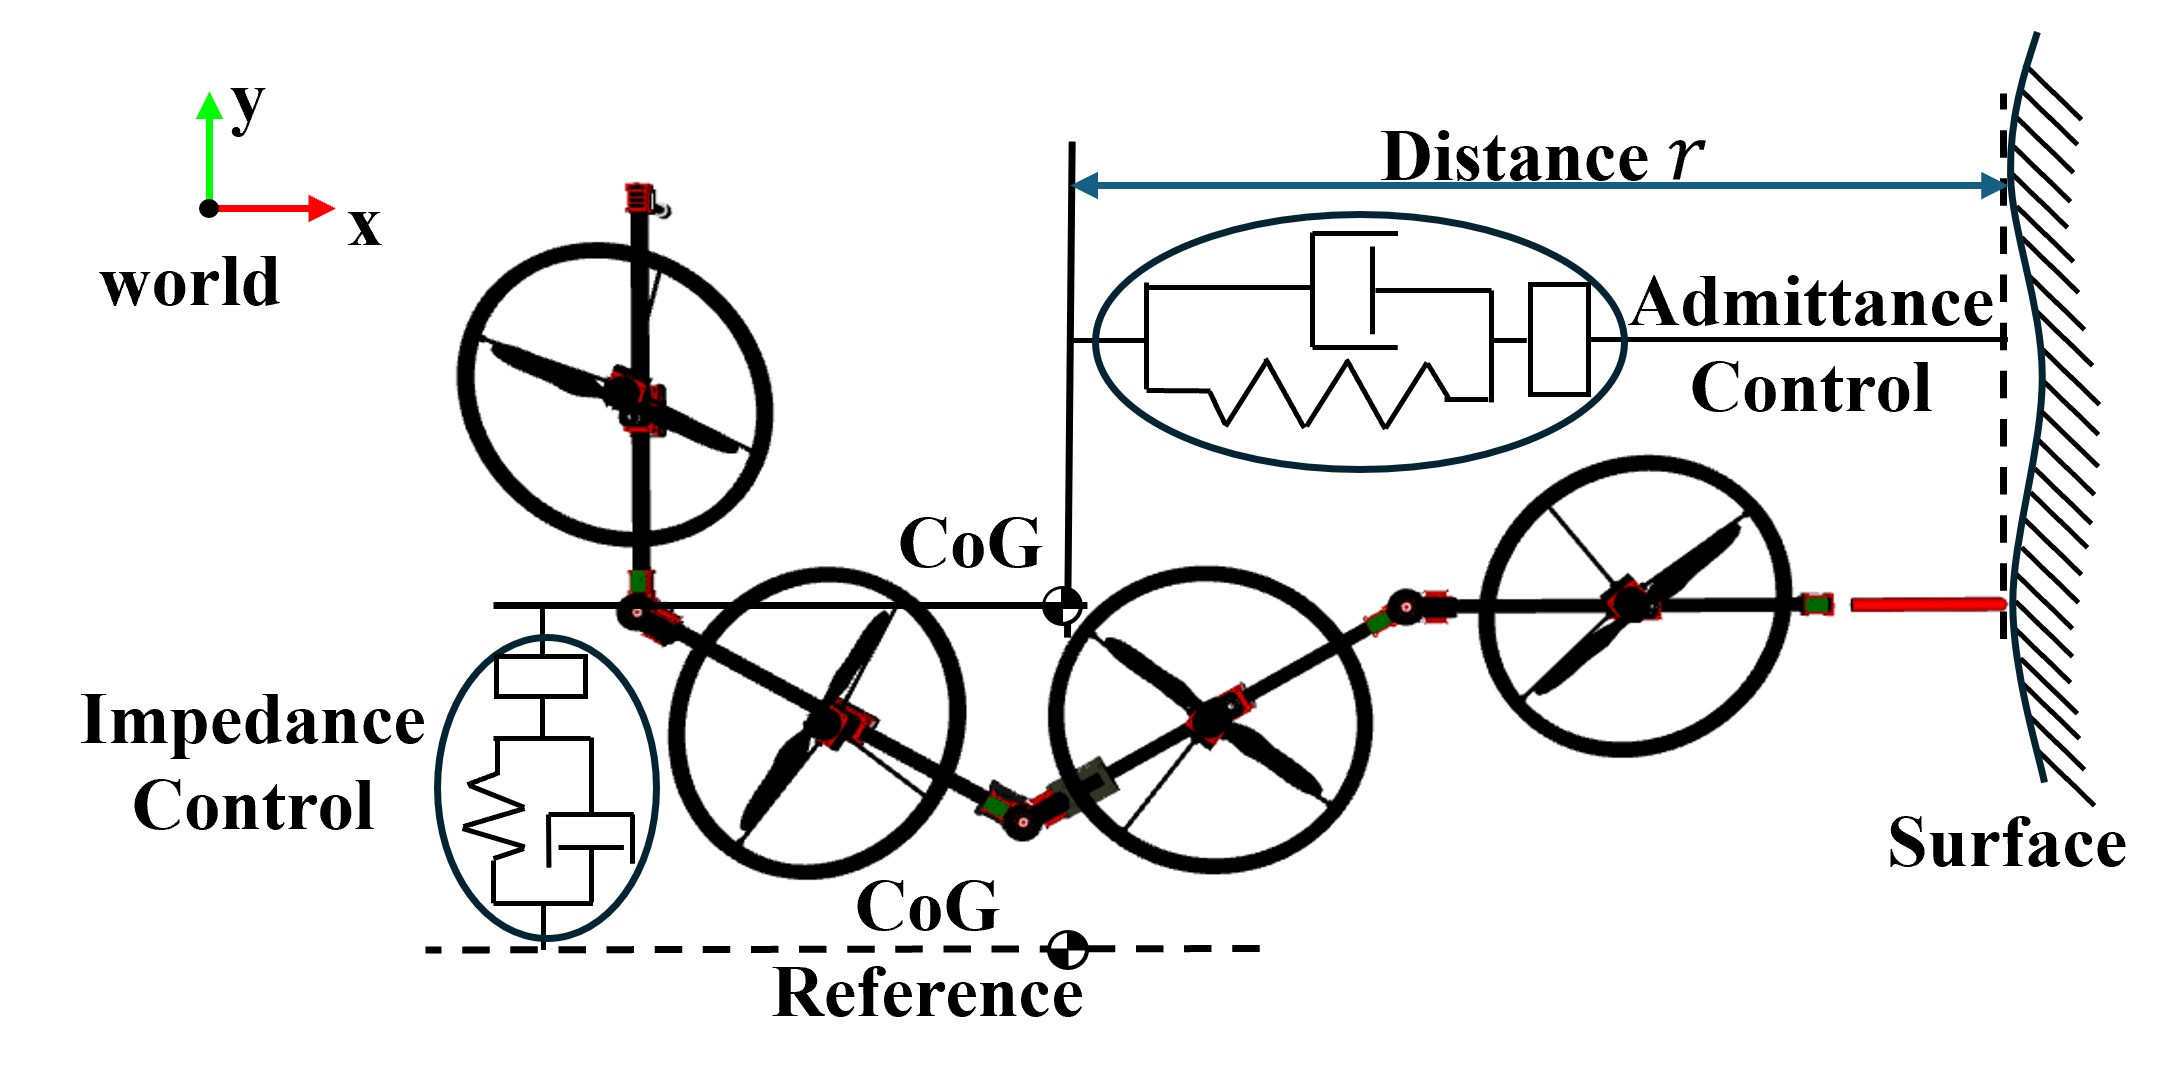
\includegraphics[trim={0cm 0.3cm 0cm 0cm}, clip,width=\linewidth]{figures/chapter3/hybrid.png}
%     \caption{Schematic diagram of the hybrid impedance-admittance control.}
%     \label{fig:hybrid_controller}
%     \vspace{-5mm}
% \end{figure}
\begin{figure}[h]
    \centering
    % \parbox{3in}
    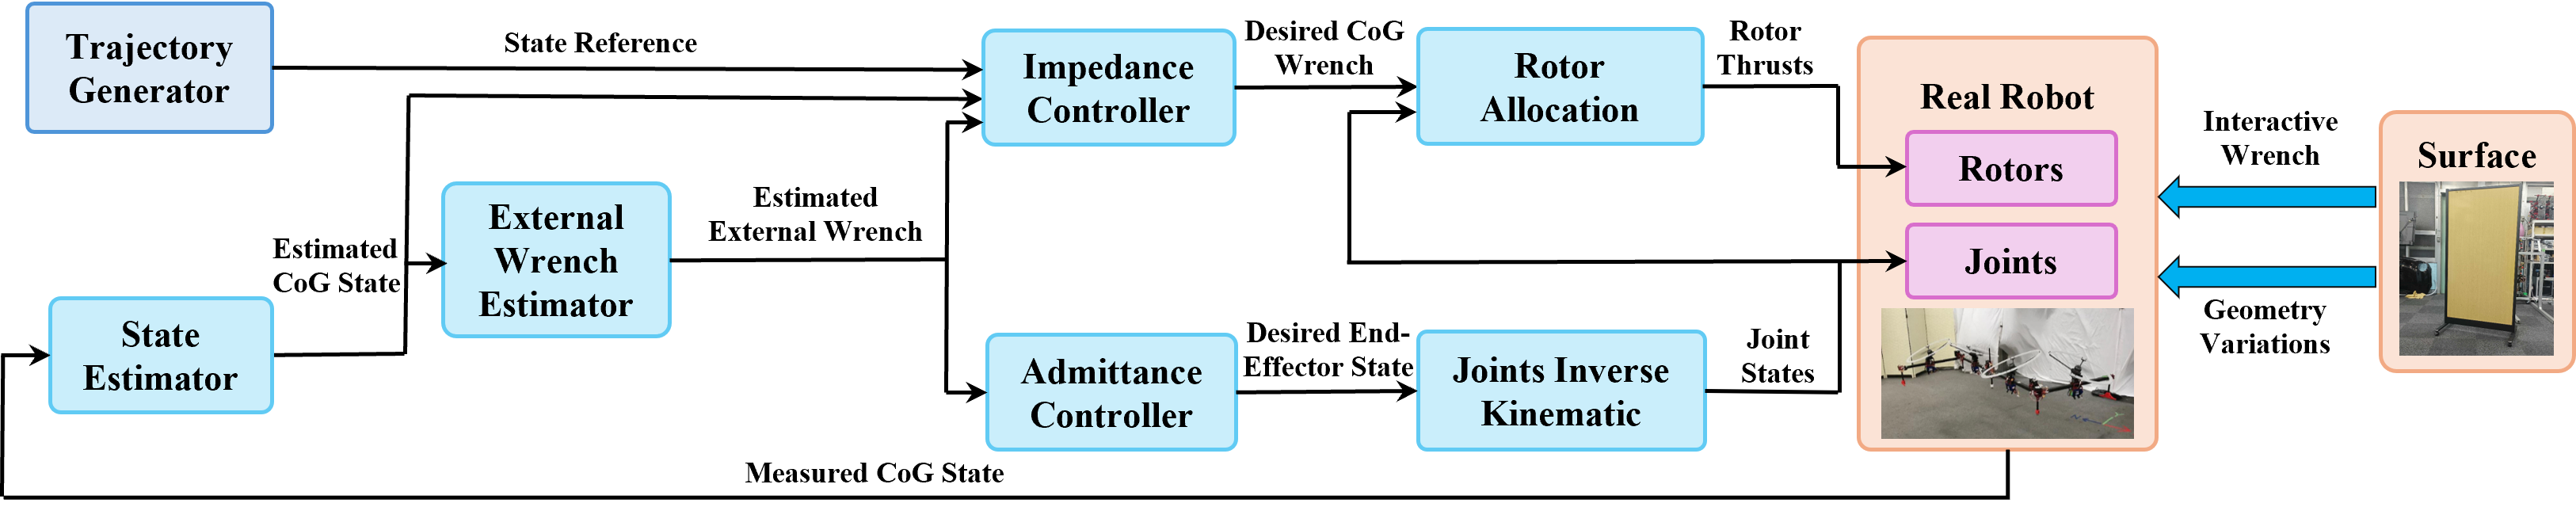
\includegraphics[trim={0cm 0.3cm 0cm 0cm}, clip,width=\linewidth]{figures/chapter3/framework.png}
    \caption{Block diagram of the hybrid impedance-admittance control framework. Inputs for the admittance controller consist of the estimated external wre
    nch. Inputs for the impedance controller include the state reference, estimated CoG state, and estimated external wrench.}
    \label{fig:framework}
    \vspace{-5mm}
\end{figure}

The motivation for this hybrid impedance-admittance control framework is to provide both resilience and adaptivity when sliding on an unknown surface, where geometry and friction introduce significant uncertainties. As illustrated in Fig.~\ref{fig:framework}, impedance control manages the overall state of the aerial robot, which is represented by the pose of its CoG, while admittance control is applied to regulate the end-effector state, resulting in adjustment of the joint angles. Since variations in joint angles modify the robot’s configuration and thus influence the thrust allocation, this dependency is taken into account in the thrust computation.
As illustrated in Fig.~\ref{fig:hybrid_controller}, by combining both controllers, the multi-link aerial robot can regulate its interaction with the surface in both force and position. Detailed analysis of the advantages of this hybrid control is presented in the following section.

%%%%%%%%%%%%%%%%%%%%%%%%%%%%%%%%%%%%%%%%%%%%%%%%%%%%%%%%%%%%%%%%%%%%%%%%%%%%%%%%
\section{External Wrench Estimation}

For both impedance control and admittance control, an external wrench is required in their respective formulations. We can choose to use force sensor to get the measured wrench data, or use estimation method to get a estimated wrench data. Generally, a force sensor is usually could only measure the external wrench applied on where it mounted. On the other hand, the estimation method can deal with force added in anywhere on the aerial robot, but it could distinguish which type of wrench. Considering the framework, the impedance control need to deal with force from different directions added in different point, so we finally choose to use estimated method.

In this framework, a momentum-based external wrench estimation method introduced in \cite{ruggiero_2014_impedance}. The wrench applied at the CoG is obtained as follows:

\begin{subequations}
\label{eq:external wrench estimation}
\begin{align}
 {^W\!\boldsymbol{\tilde{f}}_{ext}}=\boldsymbol{K}_{ti}(m^W\!\dot{\boldsymbol{p}}-\int({^W\!\boldsymbol{f}_{cmd}}-m\boldsymbol{g}+ {^W\!\boldsymbol{\tilde{f}}_{ext}})\mathrm{d}t),\\
 {^C\!\boldsymbol{\tilde{\tau}}_{ext}}=\boldsymbol{K}_{ri}(\boldsymbol{I}^C\!\boldsymbol{\omega}-\int({^C\!\boldsymbol{\tau}_{cmd}}-{^C\!\boldsymbol{\omega}} \times \boldsymbol{I}{^C\!\boldsymbol{\omega}} + {^C\!\boldsymbol{\tilde{\tau}}_{ext}})\mathrm{d}t),
\end{align}
\end{subequations}
where ${^W\!\boldsymbol{\tilde{f}}_{ext}}$ is the estimated external force, ${^C\!\boldsymbol{\tilde{\tau}}_{ext}}$ is the estimated external torque, and they can be assumed to be equal to the real external force ${^W\!\boldsymbol{f}}_{ext}$ and the real external torque   ${^C\!\boldsymbol{\tau}_{ext}}$, respectively. $\boldsymbol{K}_{ti} \in \mathbb{R}^{3\times3} \in $ and $\boldsymbol{K}_{ri} \in \mathbb{R}^{3\times3}$ are the estimator translation gain matrix and estimator rotation gain matrix, respectively.

Differentiating (\ref{eq:external wrench estimation}) and substituting (\ref{eq:dynamics}) into it yields a first-order low-pass filtered form: 
\begin{subequations}
\label{eq:external wrench estimation low-pass}
\begin{align}
 {^W\!\boldsymbol{\dot{\tilde{f}}}_{ext}}&=\boldsymbol{K}_{ti}({^W\!\boldsymbol{f}}_{ext}-{^W\!\boldsymbol{\tilde{f}}_{ext}}),\\
 {^C\!\boldsymbol{\dot{\tilde{\tau}}}_{ext}}&=\boldsymbol{K}_{ri}({^C\!\boldsymbol{\tau}_{ext}}-{^C\!\boldsymbol{\tilde{\tau}}_{ext}}).
\end{align}
\end{subequations}
That means by increasing the parameters, the estimated data will follow the real data faster, but also easier to introduce noise and lead to instability.

Note that \eqref{eq:external wrench estimation} estimates external forces and torques without using acceleration measurements, relying solely on the estimated linear and angular velocities. That means only by using built-in IMU data, we can realize getting the external wrench data.


%%%%%%%%%%%%%%%%%%%%%%%%%%%%%%%%%%%%%%%%%%%%%%%%%%%%%%%%%%%%%%%%%%%%%%%%%%%%%%%%
\section{Impedance Control}
Impedance control models the robot as a second-order system in the sight of environment, so that the robot can adjusting its own movement by external force. To meat different requirements, the dynamic parameters can be freely designed to achieve the desired interaction behavior.
For example, by adjusting the stiffness parameters, the robot can be made resilient in certain directions to reject disturbances while remaining compliant in others to maintain safe interaction \cite{bodie_2020_active}. By using impedance control, we can redesign how the system performs. In this section, we will introduce the normal concept of impedance control, also discuss about the fundamental concept of impedance control, and the difference between the PID control and it. 
% In this section, we will introduce how to adjust parameters to make the aerial robot to meet the require performance.
% In this subsection, we will introduce the 
\subsection{Normal setup}
First we will introduce how to get the command wrench equation of impedance control.
The translational motion is expressed in the world frame $\{W\}$, whereas the rotational motion is expressed in the CoG frame $\{C\}$. Under this convention, the impedance equations are written as:
\begin{subequations}
\label{eq:impedance control 1}
\begin{align}
    {\boldsymbol{M}_{d}}{^W\!\ddot{\boldsymbol{p}}}+{\boldsymbol{C}_{td}}{\boldsymbol{e}_v}+{\boldsymbol{K}_{td}}{\boldsymbol{e}_p}&={^W\!\boldsymbol{\tilde{f}}_{ext}}, \\[2pt]
    {\boldsymbol{I}_{d}}{^C\!\dot{\boldsymbol{\omega}}}+{\boldsymbol{C}_{rd}}{\boldsymbol{e}_\omega}+{\boldsymbol{K}_{rd}}{\boldsymbol{e}_R}&={^C\!\boldsymbol{\tilde{\tau}}_{ext}},
\end{align}
\end{subequations}
where ${\boldsymbol{M}_{d}}\in \mathbb{R}^{3\times3}$ is the desired virtual mass, ${\boldsymbol{I}_{d}}\in \mathbb{R}^{3\times3}$ is the desired virtual inertia, ${\boldsymbol{C}_{td}}\in \mathbb{R}^{3\times3}$, ${\boldsymbol{C}_{rd}}\in \mathbb{R}^{3\times3}$ are the desired linear and rotational damping matrices, and ${\boldsymbol{K}_{td}}\in \mathbb{R}^{3\times3}$, ${\boldsymbol{K}_{rd}}\in \mathbb{R}^{3\times3}$ are the desired linear and rotational stiffness matrices, respectively. All of these matrices are positive definite. These are what we want the system performs like. Here the error vectors in (\ref{eq:impedance control 1}) are defined as:
\begin{subequations}
\label{eq:error of rotation}
\begin{align}
    {\boldsymbol{e}_p}&={^W\!\boldsymbol{p}}-{^W\!\boldsymbol{p}_{ref}}, \\[2pt]
    {\boldsymbol{e}_v}&={^W\!\dot{\boldsymbol{p}}}-{^W\!\dot{\boldsymbol{p}}_{ref}}, \\[2pt]
    {\boldsymbol{e}_R}&=\frac{1}{2}({^W\!\boldsymbol{R}^{\mathrm{T}}_{C,ref}}{^W\!\boldsymbol{R}_{C}}-{^W\!\boldsymbol{R}^{\mathrm{T}}_{C}}{^W\!\boldsymbol{R}_{C,ref}})^\vee, \\[2pt]
    {\boldsymbol{e}_\omega}&={^C\!\boldsymbol{\omega}}-{^W\!\boldsymbol{R}^{\mathrm{T}}_{C}}{^W\!\boldsymbol{\omega}}_{ref},
\end{align}
\end{subequations}
where we use the vee-operator $^\vee$ to extract a vector from a skew symmetric matrix.

Next, by substituting \eqref{eq:dynamics} into \eqref{eq:impedance control 1} to eliminate $\ddot{\boldsymbol{p}}$ and $\dot{\boldsymbol{\omega}}$, the command wrench added on the CoG can be derived. The translational component can be written as

\begin{equation}
\label{eq:imp cmd for trans1}
    {^W\!\boldsymbol{f}_{cmd}}=(m\boldsymbol{M}^{-1}_d-\boldsymbol{E}_3){^W\!\boldsymbol{\tilde{f}}_{ext}}-m\boldsymbol{M}_d^{-1}({\boldsymbol{C}_{td}}{\boldsymbol{e}_v}+{\boldsymbol{K}_{td}}{\boldsymbol{e}_p})+m\boldsymbol{g}.
\end{equation}

And the rotational component can be written as

\begin{equation}
\label{eq:imp cmd for rot1}
    {^{C}\boldsymbol{\tau}_{cmd}}=(\boldsymbol{I}\boldsymbol{I}^{-1}_d-\boldsymbol{E}_3){^{C}}\boldsymbol{\tilde{\tau}}_{ext}-\boldsymbol{I}\boldsymbol{I}^{-1}_d({\boldsymbol{C}_{rd}}{\boldsymbol{e}_\omega}+{\boldsymbol{K}_{rd}}{\boldsymbol{e}_R})+{^{C}\boldsymbol{\omega}} \times \boldsymbol{I}{^{C}\boldsymbol{\omega}}.
\end{equation}
 
\subsection{Parameter tuning discussion}
Apparently, the performance of aerial robot is relied on the parameter matrices. Even though the parameter matrices usually have specific physical meaning, these physical interpretations do not directly provide a practical parameter selection procedure. Therefore, although the qualitative influence of each parameter is generally understood, determining suitable numerical values remains difficult in practice. 

In this thesis, the impedance parameters are analyzed according to the resulting system behavior rather than their physical meanings alone. We can find some relationship between PID control and impedance control, therefore use PID inspired tuning method to find the suitable parameters. We will use 1-dof system to explain it.

Let's consider the following 1-dof impedance control equation
\begin{equation}
\label{eq:imp cmd analysis1}
  m_d\ddot{p}+c_de_v+k_de_p = f_{ext},
\end{equation}
Here, the parameters $m_d$, $c_d$, $k_d$ are the designed mass, the designed damping, and the designed stiffness, respectively. $f_{ext}$ represents the external force.
The dynamic equation of a 1-dof object
\begin{equation}
\label{eq:imp cmd analysis2}
  m\ddot{p}+g(\dot{p}, p) = f_{ext},
\end{equation}
here $g(\dot{p}, p)$ represents an extreme term such as gravity and Coriolis.
By substituting \ref{eq:imp cmd analysis2} into \ref{eq:imp cmd analysis1}, we can get

\begin{equation}
\label{eq:imp cmd analysis3}
{{f}_{cmd}}=(\frac{m}{m_d}-1){{f}_{ext}}-m({\frac{c_d}{m_d}e_v+\frac{c_d}{k_d}e_p})+g(\dot{p}, p).
\end{equation}

Theoretically, the three parameters can be chosen independently refer to the task requirement. 
we define $\tilde{c}_d = \frac{c_d}{m_d}$, $\tilde{k}_d = \frac{k_d}{m_d}$ as the normalized damping and normalized stiffness, respectively. we use $\mu$ to replace $\frac{m}{m_d}$, so the equation becomes 
\begin{equation}
\label{eq:imp cmd analysis4}
{{f}_{cmd}}=(\mu-1){{f}_{ext}}-m({\tilde{c}_de_v+\tilde{k}_de_p})+g(\dot{p}, p).
\end{equation}

If we write the PID control equation 
\begin{equation}
\label{eq:PID cmd}
{{f}_{cmd}}=k_pe_p+k_i\int e_p\mathrm{d}t+k_de_v+g(\dot{p}, p),
\end{equation}
We will find that the two equations are very similar. If we chose $\tilde{c}_d=-\frac{k_d}{m}$ and $\tilde{k}_d=-\frac{k_p}{m}$, the only different lines on the I term $k_i\int e_p\mathrm{d}t$ and the external force term $(\mu-1){{f}_{ext}}$. 

When there exists position error, the I term $k_i\int e_p\mathrm{d}t$ will continue integral to increase the command force. If there is free flight situation, maybe it would not cause problem. But if there exists a non-zero external force, the integral term will increase to infinite except we set a limitation in advance. That is means the integral term unable to respond well to external forces. On the other hand, the external force term $(\mu-1){{f}_{ext}}$ is related to the estimated external force. It can adjust the final command wrench by considering the external force. Therefore, in the contact scenario, it is better to choose impedance control instead of PID control.
% Obviously, they all used for compensate the position errors.
% Let see what will happen in different scenarios. 

However, the impedance control still has a lot of similarities to the PID control. So we can divide it into PD control part and external force part. Apparently, if there is no external force, the external force part should disappear, and only PD control part (also the gravity part which should be considered as feedforward term) left. So we can use PID turning method to find the parameters $\tilde{c}_d$ and $\tilde{k}_d$, now they are consider as the $k_p$ and $k_d$.

After we tuning the parameters in free flight, it must be consider in contact situation. Let us consider the parameter $\mu$. If $\mu$ is set to $0$, the compensation term is exactly the estimated external wrench, so the command will completed compensate the external force. If $\mu$ is set to $1$, the external force term will also disappear, in which situation the impedance controller degenerate to a PD controller. If $\mu >1$, the external force term has the same direction with the external force, so the command will help to push the aerial robot to the direction of external force, which means the aerial robot will follow the external force. In this situation, the aerial robot can be regarded as compliance, the stiffness is relatively low. On the other hand, if $\mu >1$, the external force term has the reverse direction with the external force, which means the command will help to resist the external force. In this situation, the aerial robot will try to reduce its movement at the direction of external force, the stiffness is relatively high. 

In summary, by setting $\mu$ larger or less than $1$, the aerial robot can perform relatively compliant or rigid. By tuning parameters depend on the task requirements and environment situation, the aerial robot can perform differently in each axis. 
% The impedance control usually set the parameter between $0$ and $\inf$. If the parameter

And we can also get the tuning principle as follow. We can first tune $\tilde{c}_d$ and $\tilde{k}_d$ as the PD controller in free flight, the design the value of $\mu$ to realize what the task what to achieve. Because we use the same set of parameters both in free flight and contact, it is not necessary to switch mode before and after contacting.

% This is how we can get the command force and torque.

% The reason we rewrite the equations is that we can consider it in another way.
% The equation can be considered as being consist of three parts: the pure PD control term $-m({\tilde{c}_de_v+\tilde{k}_de_p})$, the compensation term $(\mu-1){{f}_{ext}}$ and the extreme term $g(e_v, e_p)$
So in this insight, the impedance control can be consider as the upper lever of pure PD control and feedforward + PD control, or we can also consider the equation as PID controller whose integral term is replaced by estimated wrench term \cite{bodie_2023_omnidirectional}. If the parameter is set to $1$, the compensation term disappeared, and the equation di to pure PD control. By adjusting $\mu$, the performance will be different, and satisfy the requirements of tasks.





% So actually we use the same parameters whatever the drone is in free flight or in contacting. when contact happen, the equation will use the compensation term to help deal with the external force.
% \eqref{eq:imp cmd for trans1} and 

% If there is static force added in the aerial robot, such as force disturbance. For PID controller, the I term will help to resist the external force, so finally the position errors will disappear. For impedance controller, the external term usually could not completely resist the external force, so there must be position errors remained. But the position error can be reduced by tuning the parameter $\mu$. 
%%%%%%%%%%%%%%%%%%%%%%%%%%%%%%%%%%%%%%%%%%%%%%%%%%%%%%%%%%%%%%%%%%%%%%%%%%%%%%%%
% \section{Parameter analysis}
% In most of the pervious paper using impedance control in aerial manipulation, impedance control is usually used as a tool without being entirely explained. Here we will try to explain it.
% The impedance control equation usually has three parameters to tune. By unit setting, we can rewrite the equation, and discover the insight of the equation.




% %%%%%%%%%%%%%%%%%%%%%%%%%%%%%%%%%%%%%%%%%%%%%%%%%%%%%%%%%%%%%%%%%%%%%%%%%%%%%%%%
% \subsection{Free flight}
% In free flight.
% If there is no force, the two controllers performs similar.
% If there is static force added in the aerial robot, such as force disturbance. For PID controller, the I term will help to resist the external force, so finally the position errors will disappear. For impedance controller, the external term usually could not completely resist the external force, so there must be position errors remained. But the position error can be reduced by tuning the parameter $\mu$. 
% \subsection{Contact}
% In contact state. 
\subsection{Special setup}



Finally, we can rewrite the \ref{eq:imp cmd for trans1} and \ref{eq:imp cmd for rot1} as follow.  Here we define the normalized linear damping and stiffness as $\tilde{\boldsymbol{C}}_{td} = \boldsymbol{M}^{-1}_d\boldsymbol{C}_{td}$ and $\tilde{\boldsymbol{K}}_{td} = \boldsymbol{M}^{-1}_d\boldsymbol{K}_{td}$, respectively. Using these definitions, \eqref{eq:imp cmd for trans1} can be rewritten as
\begin{equation}
\label{eq:imp cmd for trans2}
    {^W\!\boldsymbol{f}_{cmd}}=(m\boldsymbol{M}^{-1}_d-\boldsymbol{E}_3){^W\!\boldsymbol{\tilde{f}}_{ext}}-m(\tilde{\boldsymbol{C}}_{td}{\boldsymbol{e}_v}+{\tilde{\boldsymbol{K}}_{td}}{\boldsymbol{e}_p})+m\boldsymbol{g}.
\end{equation}
Also we define the normalized rotation damping and stiffness as $\tilde{\boldsymbol{C}}_{rd} = \boldsymbol{I}^{-1}_d\boldsymbol{C}_{rd}$ and $\tilde{\boldsymbol{K}}_{rd} = \boldsymbol{I}^{-1}_d\boldsymbol{K}_{rd}$, respectively. Equation (\ref{eq:imp cmd for rot1}) can then be rewritten as
\begin{equation}
\label{eq:imp cmd for rot2}
    {^{C}\boldsymbol{\tau}_{cmd}}=(\boldsymbol{I}\boldsymbol{I}^{-1}_d-\boldsymbol{E}_3){^{C}}\boldsymbol{\tilde{\tau}}_{ext}-\boldsymbol{I}(\tilde{\boldsymbol{C}}_{rd}{\boldsymbol{e}_\omega}+\tilde{\boldsymbol{K}}_{rd}{\boldsymbol{e}_\alpha})
    +{^{C}\boldsymbol{\omega}} \times \boldsymbol{I}{^{C}\boldsymbol{\omega}}.
\end{equation}
Noting that the normalized matrices are considered as contact parameters and are tuned in free flight situation. This is how we get the command wrench.

%%%%%%%%%%%%%%%%%%%%%%%%%%%%%%%%%%%%%%%%%%%%%%%%%%%%%%%%%%%%%%%%%%%%%%%%%%%%%%%%
\section{Admittance Control}
Similar to impedance control, admittance control also regulates the system’s response to external forces through a virtual dynamic relationship. However, impedance control generates a resisting force in response to displacement errors, whereas admittance control directly produces a compliant displacement in response to external forces. In this work, we employ admittance control to regulate the end-effector state by adjusting the joint angles in response to the external forces induced by surface geometric variations, thereby mitigating both the force and position disturbances experienced by the CoG through deformation.  The admittance dynamics can then be written as:


% For the surface-sliding task considered, we define the $x$ axis of the world frame as the contact direction, while the $y$ and $z$ axes represent the sliding directions. Since both the environmental contact forces and geometric variations occur primarily along the contact direction, admittance control is applied only along this direction. The admittance dynamics along the $x$ axis can then be written as:
\begin{equation}
\label{eq:admittance control}
    \boldsymbol{M}_a(\boldsymbol{\ddot{r}}_{ref}-\boldsymbol{\ddot{r}})+\boldsymbol{C}_a(\boldsymbol{\dot{r}}_{ref}-\boldsymbol{\dot{r}})+\boldsymbol{K}_a(\boldsymbol{r}_{ref}-\boldsymbol{r})={\boldsymbol{\tilde{f}}_{ext}}-\boldsymbol{f}_{ref},
\end{equation}
where ${\boldsymbol{\tilde{f}}_{ext}}$ is filtered from ${^W\!\boldsymbol{f}_{ext}}$, and $\boldsymbol{f}_{ref}$ represents the reference external force. The position vector $\boldsymbol{r} \in \mathbb{R}^{3}$ is defined as a distance, the specific definition will be changed due to tasks. The reference position vector $\boldsymbol{r}_{ref}$ corresponds to the original distance.
% , and the reference velocity and acceleration are set as $\dot{r}_{ref}=0$ and $\ddot{r}_{ref}=0$, respectively.
Finally, the parameter diagonal matrices $\boldsymbol{M}_a$, $\boldsymbol{C}_a$, $\boldsymbol{K}_a \in \mathbb{R}^{3\times3}$ denotes the admittance mass, damping, and stiffness in different axes, respectively.

We then employ a discrete-time difference method to compute the distance $\boldsymbol{r}$ at each time step, denoted as $\boldsymbol{r}[k]$. The corresponding acceleration is calculated as: 
\begin{equation}
\label{eq:difference method1}
\boldsymbol{\ddot{r}}[k]=\boldsymbol{M}^{-1}_a(({\boldsymbol{\tilde{f}}_{ext}}-\boldsymbol{f}_{ref})-\boldsymbol{K}_a(\boldsymbol{r}_{ref}-\boldsymbol{r}[k-1])+\boldsymbol{C}_a\boldsymbol{\dot{r}}[k-1]).
\end{equation}
Using this acceleration, the velocity and position can be updated iteratively according to:
\begin{subequations}
\label{eq:difference method2}
\begin{align}
\boldsymbol{\dot{r}}[k]&=\boldsymbol{\dot{r}}[k-1]+\boldsymbol{\ddot{r}}[k]\Delta t, \\[2pt]
\boldsymbol{r}[k]&=\boldsymbol{r}[k-1]+\boldsymbol{\dot{r}}[k]\Delta t,
\end{align}
\end{subequations}
where $\Delta t$ is the control period.

% Given the desired end-effector pose, the corresponding angle $\theta$ that is defined in Fig.~\ref{fig:hybrid_controller} 

Given the desired end-effector pose, the joint angles are obtained by solving the inverse kinematics (IK). This configuration allows external forces to influence the relative distance.
In theory, if we choose appropriate parameters, the distance $r$ will not change rapidly, which will help to keep stable.

Actually, consider we just what to realize displacement follow by force, we can choose to change linearly. But due to the effect of admittance control, it is adjustable by changing the parameters, which means that in different situation, we can provide different performance by tuning the parameters.




%%%%%%%%%%%%%%%%%%%%%%%%%%%%%%%%%%%%%%%%%%%%%%%%%%%%%%%%%%%%%%%%%%%%%%%%%%%%%%%%
\section{Validation on Hydrus}
\subsection{Impedance control on Hydrus}
To use impedance control on Hydrus, we need do some special step. Due to Hydrus is an underactuated system, it must control the translation part and rotation part cascadely.
To obtain the desired thrust vector, we first calculate the translational command force magnitude by
\begin{equation}
\label{eq:thrust translation 1}
    f_{cmd}=(^W\!\boldsymbol{R}_{C}\boldsymbol{b}_3){^W\!\boldsymbol{f}_{cmd}},
\end{equation}
where $^{W}\boldsymbol{R}_{C}\boldsymbol{b}_3$ represents the unit vector along the $z$ axis of the CoG frame expressed in the world frame.

Next, we determine the thrust vector associated with the rotational component. By using the tranlational command, the desired roll angle $^W\!\alpha^{tgt}_x$ and desired pitch angle $^W\!\alpha^{tgt}_y$ are computed as
\begin{subequations}
\label{eq:target roll and pitch angle}
\begin{align}
    {^W\!\alpha^{tgt}_x}&=atan^{-1}(-{^W\!\bar{f}_{y,cmd}},\sqrt{{^W\!\bar{f}_{x,cmd}^2}+{^W\!\bar{f}_{z,cmd}^2}}), \\[2pt]
    {^W\!\alpha^{tgt}_y}&=atan^{-1}(^W\!\bar{f}_{x,cmd},{^W\!\bar{f}_{z,cmd}}),
\end{align}
\end{subequations}
where
\begin{equation}
\label{eq:imp cmd for trans}
    \begin{bmatrix}
^W\!\bar{f}_{x,cmd} & ^W\!\bar{f}_{y,cmd} & ^W\!\bar{f}_{z,cmd}
\end{bmatrix}^{\mathrm{T}}=R^{-1}_Z(^W\!\alpha_z)^W\!\boldsymbol{f}_{cmd}.
\end{equation}
Here, $R_Z(\cdot{})$ is a rotation matrix that only rotates along the $z$ axis with a certain angle.

Employing the computed target roll $^W\!\alpha^{tgt}_x$, target pitch $^W\!\alpha^{tgt}_y$, and the reference yaw angle $^W\!\alpha^{ref}_z$, the reference rotation matrix $^W\!R_{C,ref}$ in \eqref{eq:error of rotation} is constructed, from which the rotation error vector ${\boldsymbol{e}_R}$ is derived. 
% In near hovering condition, we also define ${\boldsymbol{e}_\alpha}$ as the vector form of ${\boldsymbol{e}_R}^\wedge$, where the hat operator $^\wedge$ converts a skew-symmetric matrix into its corresponding vector representation.

Next, we define the following allocation relationship:
\begin{equation}
\label{eq:thrust translation 2}
     \begin{bmatrix} mf_{cmd}&0&0&0\end{bmatrix}^{\mathrm{T}}=\begin{pmatrix}
\boldsymbol{Q}_{tz} \\
\boldsymbol{Q}_r
\end{pmatrix}\boldsymbol{\lambda}_t,
\end{equation}
where $\boldsymbol{Q}_{tz} \in \mathbb{R}^{1 \times 4}$ is the third row of $\boldsymbol{Q}_t$. Solving \eqref{eq:thrust translation 2} yields the translational thrust vector $\boldsymbol{\lambda}_t$. Note that the purpose of the translational command force is to counteract gravity and generate the required translational acceleration, while ensuring that it does not affect the rotational direction.

Then the rotation thrust vector can be obtained by
\begin{equation}
\label{eq:thrust rotation 1}
     \boldsymbol{\lambda}_r=\boldsymbol{Q}_r^{\dagger}{^{C}\boldsymbol{\tau}_{cmd}},
\end{equation}
where $\boldsymbol{Q}_r^{\dagger}$ is the Moore–Penrose pseudoinverse of $ \boldsymbol{Q}_r$.

Finally, the total thrust required to be generated by the rotors can be obtained as
\begin{equation}
\label{eq:thrust}
\boldsymbol{\lambda}=\boldsymbol{\lambda}_t+\boldsymbol{\lambda}_r,
\end{equation}
This gives the individual thrust values that each rotor needs to produce. 
% The detail calculated of allocation process about the thrusts can be found in \cite{zhao_2021_singularity}.

\subsection{Admittance control on Hydrus}
In Hydrus's case, we only test one direction. For the surface-sliding task considered in this study, the $x$ axis of the world frame is defined as the contact direction, while the $y$ and $z$ axes represent the sliding directions. Since the geometric variations occur primarily along the contact direction, only single-axis admittance control is employed along this direction. This design choice avoids additional structural motions in non-contact directions, which could adversely affect the stability of the aerial robot. The admittance dynamics along the $x$ axis can then be written as: 
\begin{equation}
\label{eq:admittance control2}
    m_a(\ddot{r}_{ref}-\ddot{r})+c_a(\dot{r}_{ref}-\dot{r})+k_a(r_{ref}-r)=\hat{f}_{ext,x}-f_{ref,x},
\end{equation}

\begin{equation}
\label{eq:difference method1}
\ddot{r}[k]=\frac{(\hat{f}_{ext,x}-f_{ref,x})-k_a(r_{ref}-r[k-1])+c_a\dot{r}[k-1]}{m_a}.
\end{equation}
Using this acceleration, the velocity and position can be updated iteratively according to:
\begin{subequations}
\label{eq:difference method2}
\begin{align}
\dot{r}[k]&=\dot{r}[k-1]+\ddot{r}[k]\Delta t, \\[2pt]
r[k]&=r[k-1]+\dot{r}[k]\Delta t,
\end{align}
\end{subequations}

Consequently, variations in surface geometry induce corresponding changes in the contact forces. Due to the adoption mechanism,  the majority of geometric variations and external force disturbances are absorbed at the joints, while the portion transmitted to the CoG is significantly reduced, leading to more favorable overall motion behavior of the aerial robot.
As shown in Fig.~\ref{fig:admittance_config}, we set the 2D multi-link aerial robot as the configuration to test the admittance effect. There is a rope attach at leg in joint$2$. By pulling the rope, we can imitate a external force on the negative direction of $x$ axis. As shown in Fig.~\ref{fig:admittance_changing}, the multi-link structure will change due to the external force. Fig.~\ref{fig:hybrid_controller} shows the relationship between the external force and the distance between the end effector and the CoG.


\begin{figure}[h]
    \centering
    % \parbox{3in}
    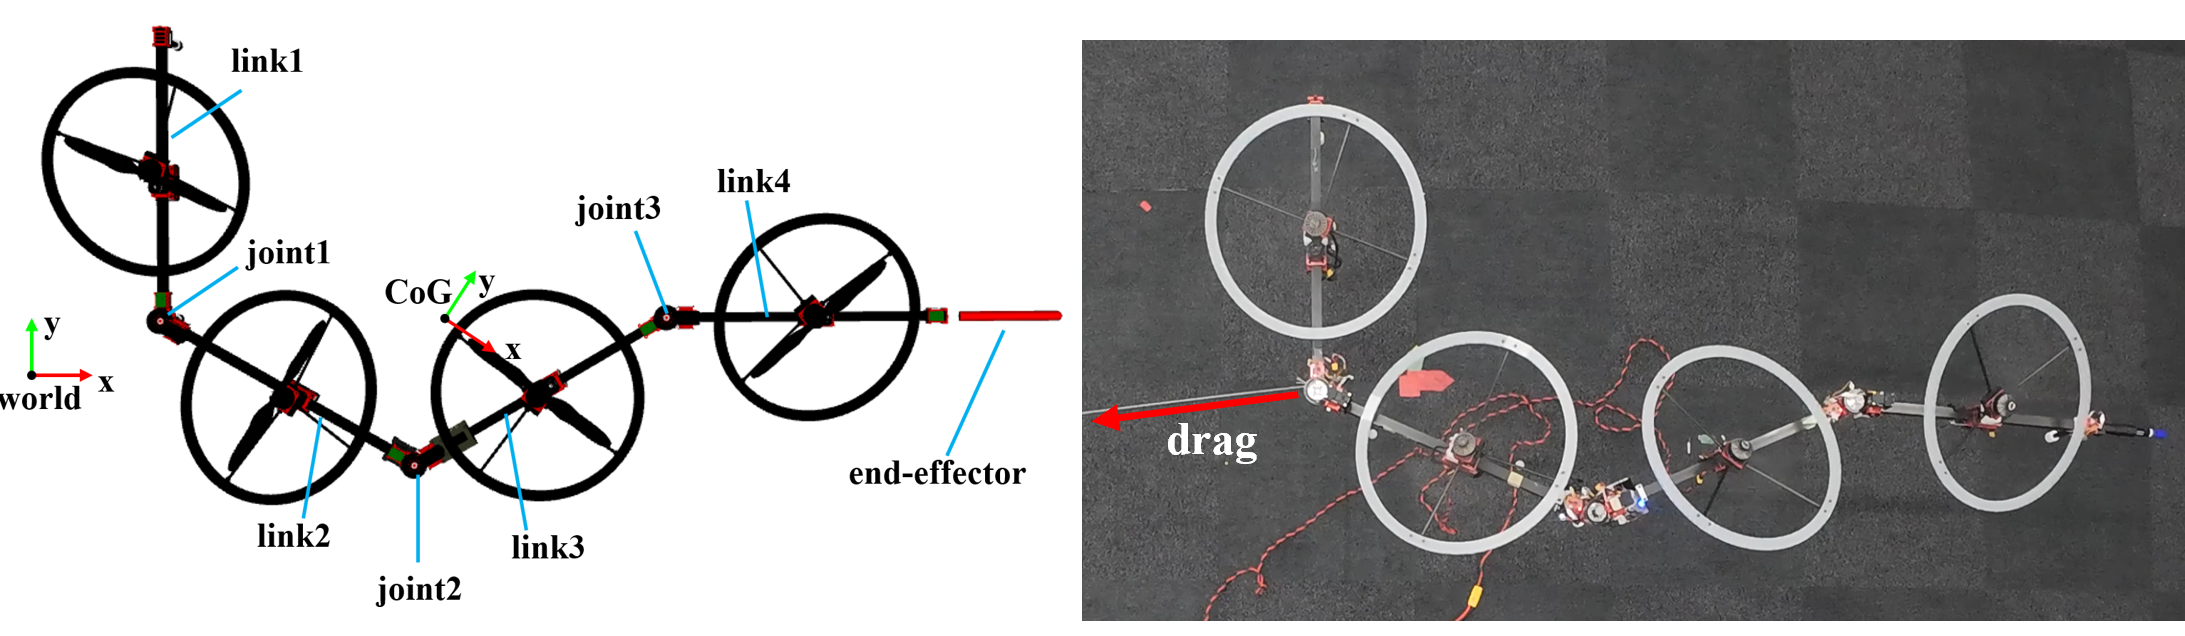
\includegraphics[trim={0cm 0.3cm 0cm 0cm},clip,width=\linewidth]{figures/chapter3/admittance_config.png}
    \caption{Admittance example configuration. Left, the model example. Right, the real machine.}
    \label{fig:admittance_config}
    \vspace{-5mm}
\end{figure}

\begin{figure}[h]
    \centering
    % \parbox{3in}
    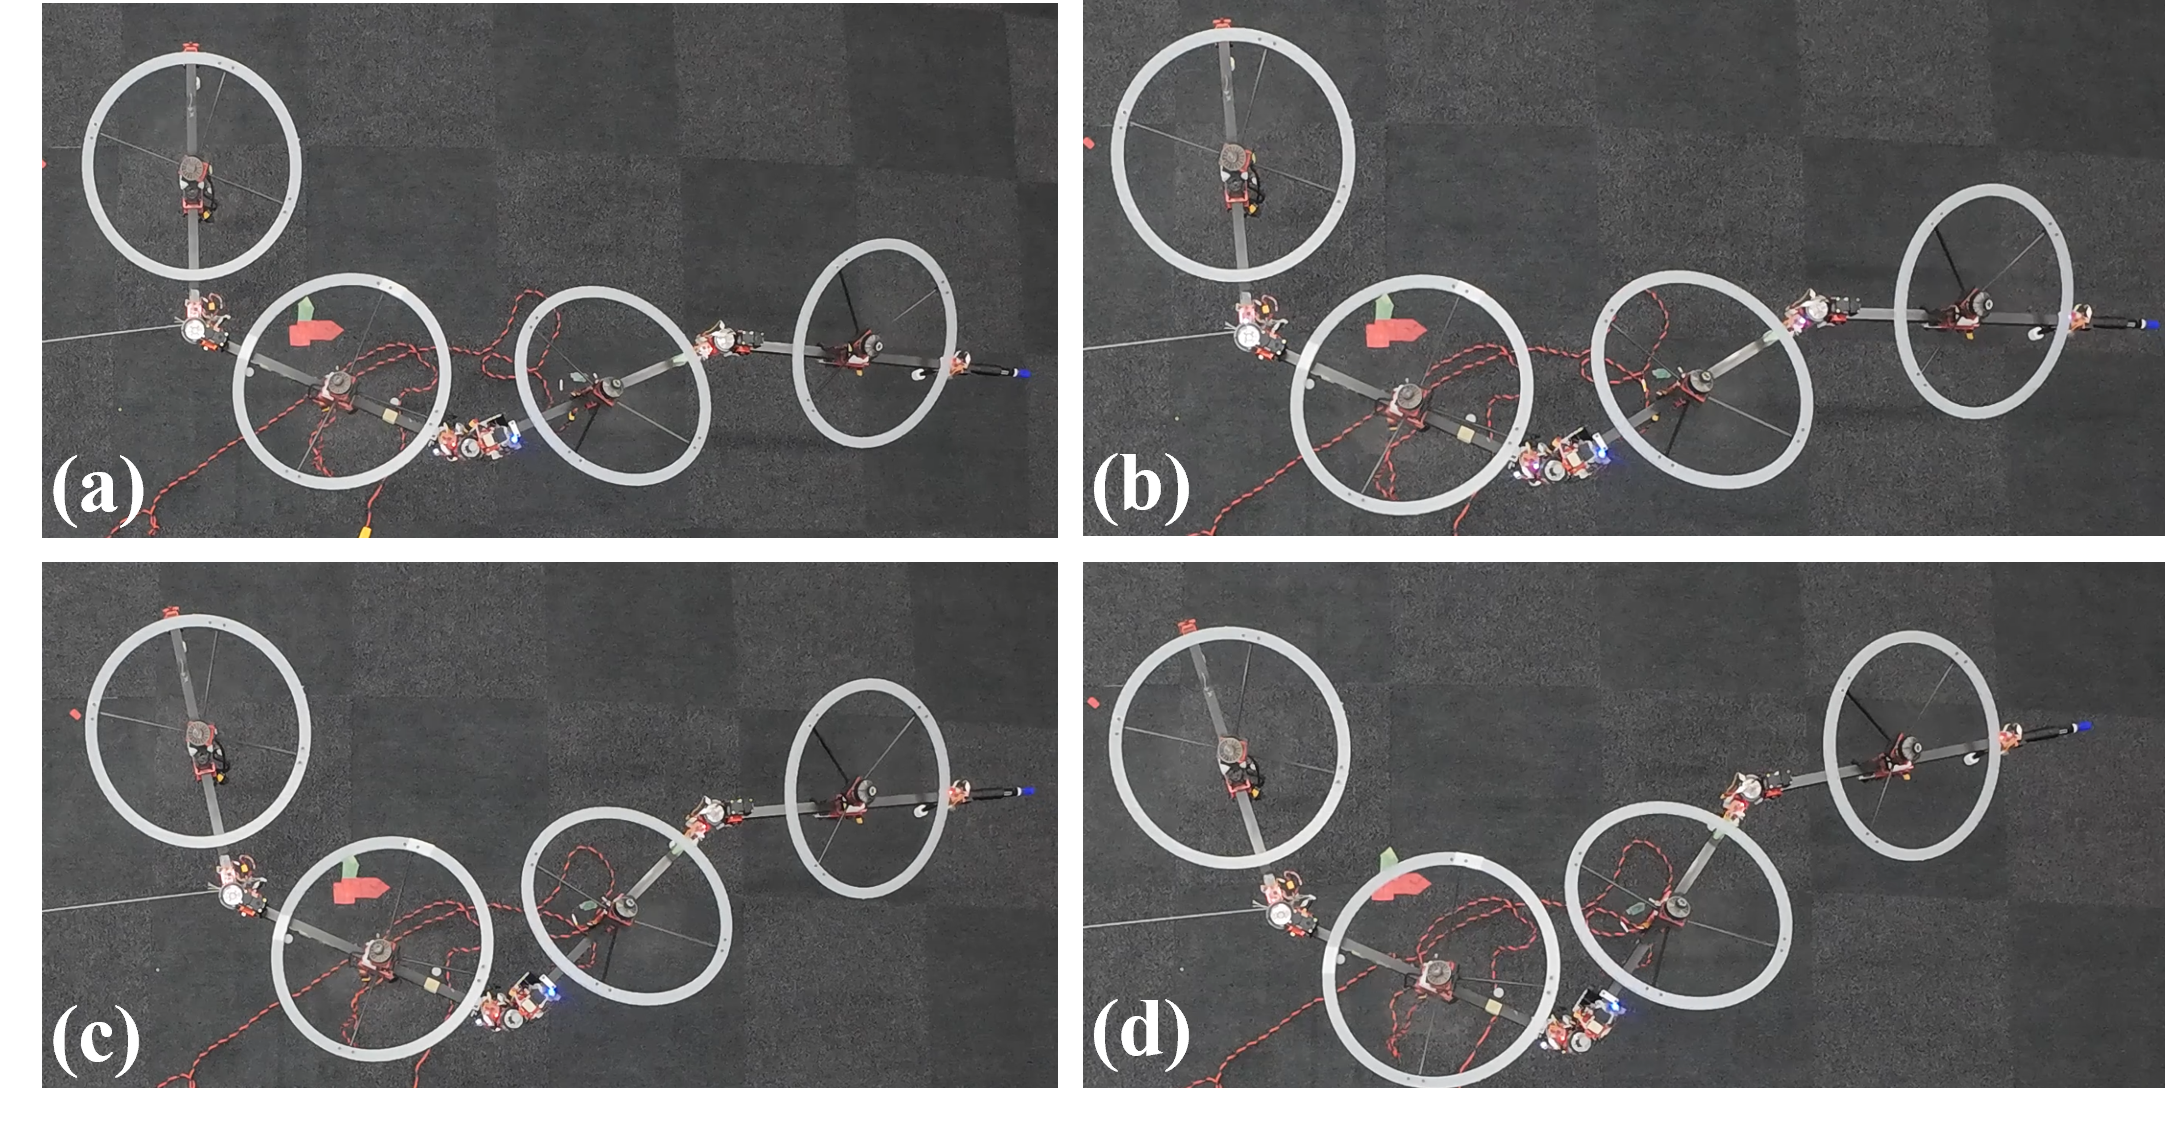
\includegraphics[trim={0cm 0.3cm 0cm 0cm},clip,width=\linewidth]{figures/chapter3/admittance_changing.png}
    \caption{(a)-(d): Admittance changing process.}
    \label{fig:admittance_changing}
    \vspace{-5mm}
\end{figure}

\subsection{Hybrid Control Mechanism} 

In surface-sliding tasks, the contact and sliding directions exhibit fundamentally different physical characteristics: the sliding directions are dominated by friction-induced disturbances, whereas the contact direction is shaped by geometric variations of the environment. Leveraging this distinction, the hybrid impedance–admittance controller assigns each axis the control behavior best suited to its interaction properties. As illustrated in Fig.~\ref{fig:hybrid_controller}, admittance control is applied along the contact direction ($x$ axis) to regulate geometry-driven variations, while impedance control governs the sliding directions ($y$ and $z$ axes) to accommodate friction-affected motion.

Through this task-aligned division of control responsibilities, the hybrid controller achieves what neither controller can provide alone: robust sliding performance in the sliding directions and adaptive behavior in the contact direction. This directional decomposition is enabled by the actuation structure of the multi-link aerial robot, which allows the two control paradigms to be realized simultaneously through independent actuation sources. This combination is therefore essential for achieving resilient interaction and adaptive contact behavior in surface-sliding tasks. The performance of the proposed hybrid impedance-admittance controller will be exhibited in the experiment chapter.

\begin{figure}[h]
    \centering
    % \parbox{3in}
    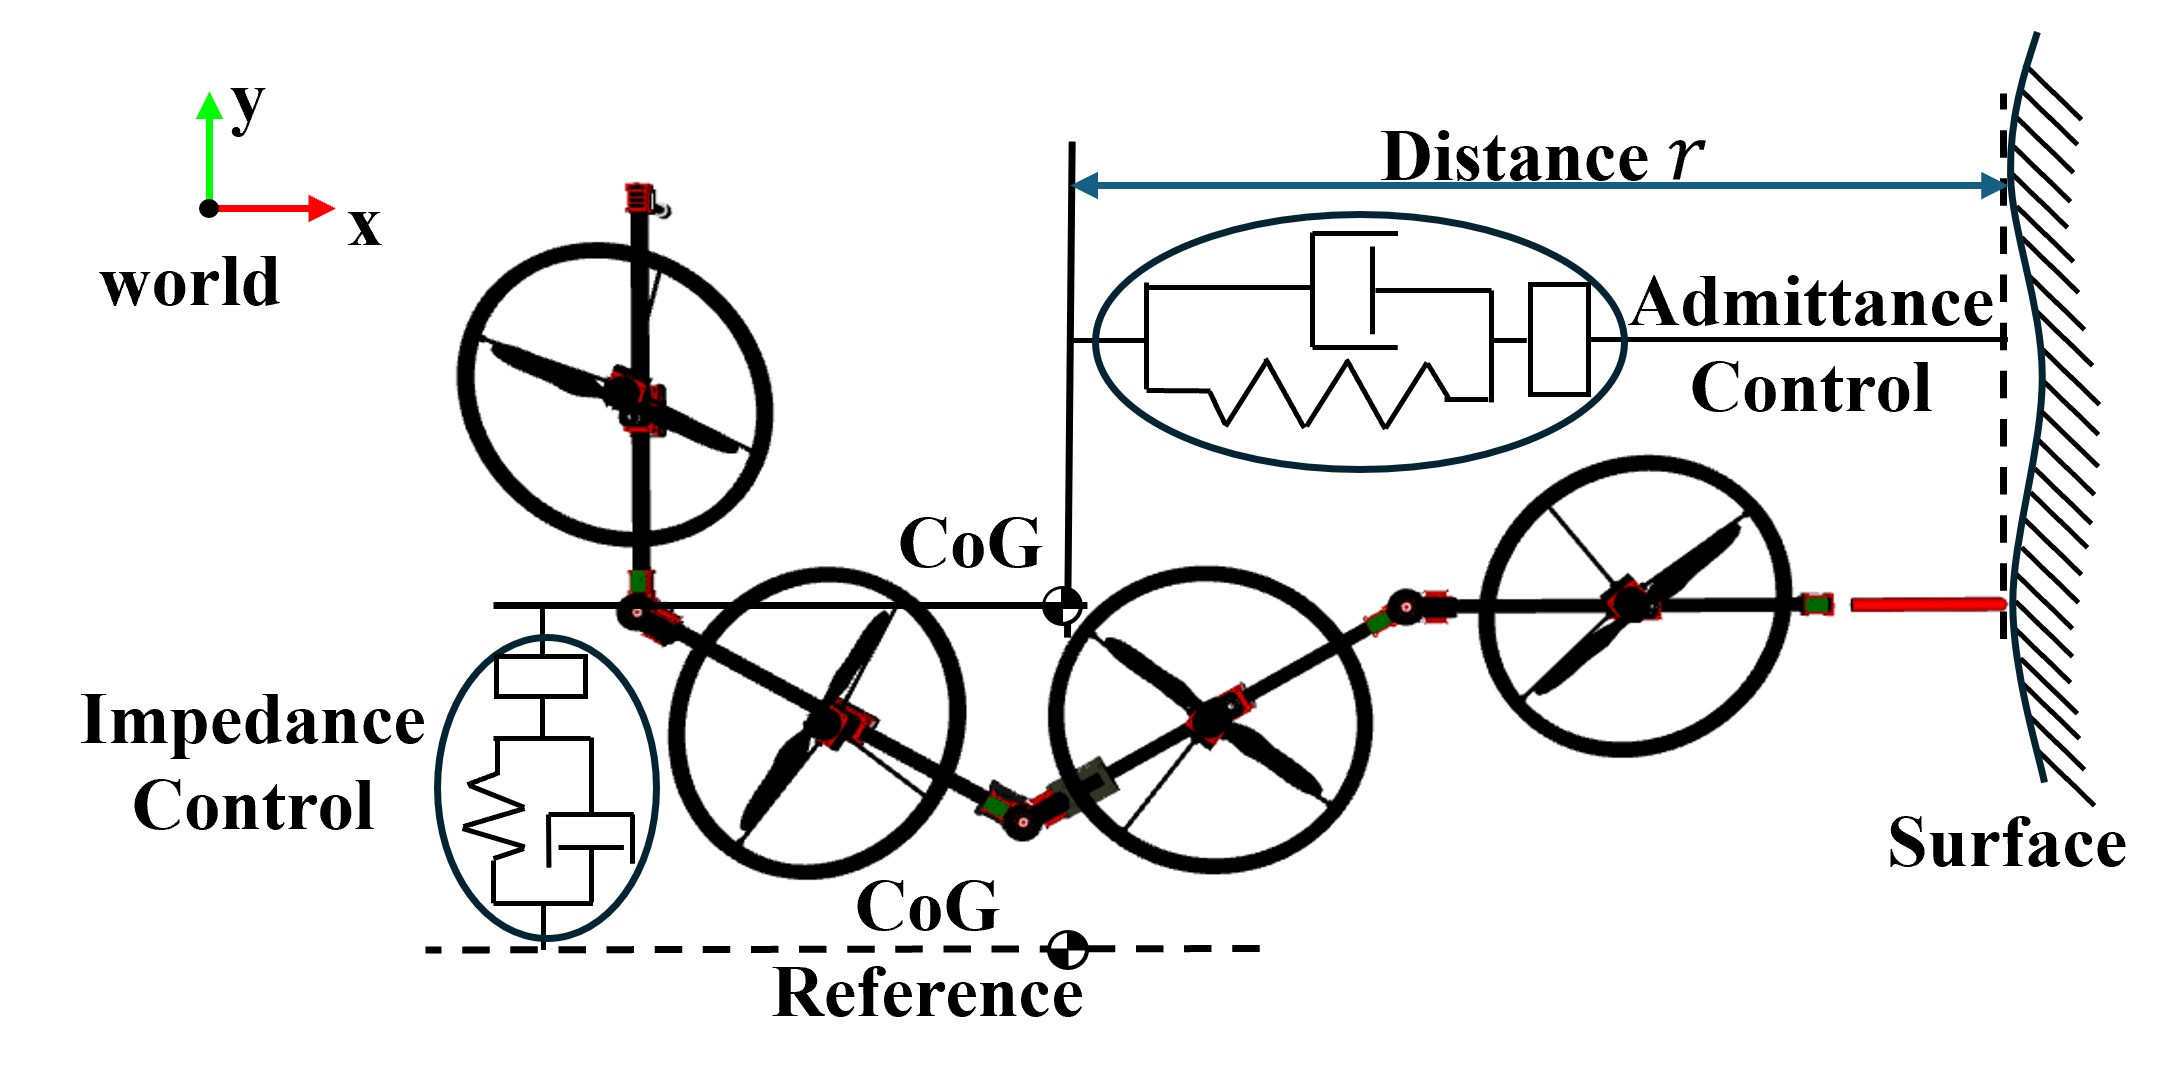
\includegraphics[trim={0cm 0.3cm 0cm 0cm},clip,width=\linewidth]{figures/chapter3/hybrid.png}
    \caption{Schematic diagram of the hybrid impedance-admittance control.}
    \label{fig:hybrid}
    \vspace{-5mm}
\end{figure}

%%%%%%%%%%%%%%%%%%%%%%%%%%%%%%%%%%%%%%%%%%%%%%%%%%%%%%%%%%%%%%%%%%%%%%%%%%%%%%%%
\section{Summary}
In this chapter. We explain that the impedance control can help to change the dynamics parameters of the system, in order to have different performances in different directions. Also, the admittance control can help to adjust the distance between the end-effector and a reference point(es tl. CoG) on the aerial robot, and help to adapt to the geometric variation of the surface. Finally, we explain both the controllers can be added together on the multi-link aerial robot and achieve the surface sliding tasks.